%%%%%%%%%%%%%%%%%%%%%%%%%%%%%%%%%%%%%%%%%
% Classicthesis Typographic Thesis
% LaTeX Template
% Version 1.4 (1/1/16)
%
% This template has been downloaded from:
% http://www.LaTeXTemplates.com
%
% Original author:
% André Miede (http://www.miede.de) with commenting modifications by:
% Vel (vel@LaTeXTemplates.com)
%
% License:
% GNU General Public License (v2)
%
% General Tips:
% 1) Make sure to edit the classicthesis-config.file
% 2) New enumeration (A., B., C., etc in small caps): \begin{aenumerate} \end{aenumerate}
% 3) For margin notes: \marginpar or \graffito{}
% 4) Do not use bold fonts in this style, it is designed around them
% 5) Use tables as in the examples
% 6) See classicthesis-preamble.sty for useful commands
%
%%%%%%%%%%%%%%%%%%%%%%%%%%%%%%%%%%%%%%%%%

%----------------------------------------------------------------------------------------
%	PACKAGES AND OTHER DOCUMENT CONFIGURATIONS
%----------------------------------------------------------------------------------------

\documentclass[
		twoside,openright,titlepage,numbers=noenddot,headinclude,%1headlines,
	 	footinclude=true,cleardoublepage=empty,
		dottedtoc, % Make page numbers in the table of contents flushed right with dots leading to them
		BCOR=5mm,paper=a4,fontsize=11pt, % Binding correction, paper type and font size
		ngerman,american, % Languages, change this to your language(s)
		]{scrreprt} 
                
% Includes the file which contains all the document configurations and packages - make sure to edit this file
%%%%%%%%%%%%%%%%%%%%%%%%%%%%%%%%%%%%%%%%%
% Classicthesis Typographic Thesis
% Configuration File
%
% This file has been downloaded from:
% http://www.LaTeXTemplates.com
%
% Original author:
% André Miede (http://www.miede.de) with extensive commenting changes by:
% Vel (vel@LaTeXTemplates.com)
%
% License:
% GNU General Public License (v2)
%
% Important note:
% The main lines to change in this file are in the DOCUMENT VARIABLES
% section, the rest of the file is for advanced configuration.
%
%%%%%%%%%%%%%%%%%%%%%%%%%%%%%%%%%%%%%%%%%

%----------------------------------------------------------------------------------------
%	CHARACTER ENCODING
%----------------------------------------------------------------------------------------

\PassOptionsToPackage{utf8}{inputenc} % Set the encoding of your files. UTF-8 is the only sensible encoding nowadays. If you can't read äöüßáéçèê∂åëæƒÏ€ then change the encoding setting in your editor, not the line below. If your editor does not support utf8 use another editor!
\usepackage{inputenc}

%----------------------------------------------------------------------------------------
%	DOCUMENT VARIABLES
%	Fill in the lines below to enter your information into the thesis template
%	Each of the commands can be cited anywhere in the thesis
%----------------------------------------------------------------------------------------

% Remove drafting to get rid of the '[ Date - classicthesis version 4.0 ]' text at the bottom of every page
\PassOptionsToPackage{eulerchapternumbers,listings,drafting, pdfspacing, subfig,beramono,eulermath,parts}{classicthesis}
% Available options: drafting parts nochapters linedheaders eulerchapternumbers beramono eulermath pdfspacing minionprospacing tocaligned dottedtoc manychapters listings floatperchapter subfig

\newcommand{\myTitle}{Non-Noble Metal Catalysts for Aerobic Cleavage of C--C Single Bonds Using Statistical Experimental Design\xspace}
\newcommand{\mySubtitle}{Cumulative Dissertation\xspace}
\newcommand{\myDegree}{\textit{doctor rerum naturalium} (Dr. rer. nat.)\xspace}
\newcommand{\myName}{David Leonard\xspace}
\newcommand{\myProf}{Prof Dr Matthias Beller\xspace}
\newcommand{\mySupervisor}{Dr Kathrin Junge\xspace}
\newcommand{\myFaculty}{Mathematics and Natural Sciences\xspace}
\newcommand{\myDepartment}{Applied Homogeneous Catalysis\xspace}
\newcommand{\myUni}{University of Rostock\xspace}
\newcommand{\myLocation}{Rostock\xspace}
\newcommand{\myTime}{July 2021\xspace}
\newcommand{\myVersion}{version 4.2\xspace}

%----------------------------------------------------------------------------------------
%	USEFUL COMMANDS
%----------------------------------------------------------------------------------------

\newcommand{\ie}{i.\,e.}
\newcommand{\Ie}{I.\,e.}
\newcommand{\eg}{e.\,g.}
\newcommand{\Eg}{E.\,g.} 

\newcounter{dummy} % Necessary for correct hyperlinks (to index, bib, etc.)
\providecommand{\mLyX}{L\kern-.1667em\lower.25em\hbox{Y}\kern-.125emX\@}
\newlength{\abcd} % for ab..z string length calculation

%----------------------------------------------------------------------------------------
%	PACKAGES
%----------------------------------------------------------------------------------------

\usepackage{lipsum} % Used for inserting dummy 'Lorem ipsum' text into the template

%------------------------------------------------

%\PassOptionsToPackage{ngerman,american}{babel}  % Change this to your language(s)
% Spanish languages need extra options in order to work with this template
%\PassOptionsToPackage{spanish,es-lcroman}{babel}
\usepackage{babel}
%\usepackage{pdfpages}
%------------------------------------------------			

\usepackage{csquotes}
\PassOptionsToPackage{%
%backend=biber, % Instead of bibtex
backend=bibtex8,bibencoding=ascii,%
language=auto,%
style=numeric-comp,%
%style=authoryear-comp, % Author 1999, 2010
%bibstyle=authoryear,dashed=false, % dashed: substitute rep. author with ---
sorting=nyt, % name, year, title
maxbibnames=10, % default: 3, et al.
%backref=true,%
natbib=true % natbib compatibility mode (\citep and \citet still work)
}{biblatex}
\usepackage[sorting=none, style = chem-acs]{biblatex}
 
 %------------------------------------------------

\PassOptionsToPackage{fleqn}{amsmath} % Math environments and more by the AMS 
 \usepackage{amsmath}
 
 %------------------------------------------------

\PassOptionsToPackage{T1}{fontenc} % T2A for cyrillics
\usepackage{fontenc}

%------------------------------------------------

\usepackage{textcomp} % Fix warning with missing font shapes

%------------------------------------------------

\usepackage{scrhack} % Fix warnings when using KOMA with listings package  

%------------------------------------------------

\usepackage{xspace} % To get the spacing after macros right

%------------------------------------------------

\usepackage{mparhack} % To get marginpar right

%------------------------------------------------

\usepackage{fixltx2e} % Fixes some LaTeX stuff 

%------------------------------------------------

\PassOptionsToPackage{smaller}{acronym} % Include printonlyused in the first bracket to only show acronyms used in the text
\usepackage{acronym} % Nice macros for handling all acronyms in the thesis

%\renewcommand*{\acsfont}[1]{\textssc{#1}} % For MinionPro
\renewcommand*{\aclabelfont}[1]{\acsfont{#1}}

%------------------------------------------------

\PassOptionsToPackage{pdftex}{graphicx}
\usepackage{graphicx} 

%----------------------------------------------------------------------------------------
%	FLOATS: TABLES, FIGURES AND CAPTIONS SETUP
%----------------------------------------------------------------------------------------

\usepackage{tabularx} % Better tables
\setlength{\extrarowheight}{3pt} % Increase table row height
\newcommand{\tableheadline}[1]{\multicolumn{1}{c}{\spacedlowsmallcaps{#1}}}
\newcommand{\myfloatalign}{\centering} % To be used with each float for alignment
\usepackage{caption}
\captionsetup{font=small}
\usepackage{subfig}  

%----------------------------------------------------------------------------------------
%	CODE LISTINGS SETUP
%----------------------------------------------------------------------------------------

\usepackage{listings} 
%\lstset{emph={trueIndex,root},emphstyle=\color{BlueViolet}}%\underbar} % For special keywords
\lstset{language=[LaTeX]Tex,%C++ % Specify the language(s) for listings here
morekeywords={PassOptionsToPackage,selectlanguage},
keywordstyle=\color{RoyalBlue}, % Add \bfseries for bold
basicstyle=\small\ttfamily, % Makes listings a smaller font size and a different font
%identifierstyle=\color{NavyBlue}, % Color of text inside brackets
commentstyle=\color{Green}\ttfamily, % Color of comments
stringstyle=\rmfamily, % Font type to use for strings
numbers=left, % Change left to none to remove line numbers
numberstyle=\scriptsize, % Font size of the line numbers
stepnumber=5, % Increment of line numbers
numbersep=8pt, % Distance of line numbers from code listing
showstringspaces=false, % Sets whether spaces in strings should appear underlined
breaklines=true, % Force the code to stay in the confines of the listing box
%frameround=ftff, % Uncomment for rounded frame
%frame=single, % Frame border - none/leftline/topline/bottomline/lines/single/shadowbox/L
belowcaptionskip=.75\baselineskip % Space after the "Listing #: Desciption" text and the listing box
}

%----------------------------------------------------------------------------------------
%	HYPERREFERENCES
%----------------------------------------------------------------------------------------

\PassOptionsToPackage{pdftex,hyperfootnotes=false,pdfpagelabels}{hyperref}
\usepackage{hyperref}  % backref linktocpage pagebackref
\pdfcompresslevel=9
\pdfadjustspacing=1

\hypersetup{
% Uncomment the line below to remove all links (to references, figures, tables, etc), useful for b/w printouts
%draft, 
colorlinks=true, linktocpage=true, pdfstartpage=3, pdfstartview=FitV,
% Uncomment the line below if you want to have black links (e.g. for printing black and white)
%colorlinks=false, linktocpage=false, pdfborder={0 0 0}, pdfstartpage=3, pdfstartview=FitV, 
breaklinks=true, pdfpagemode=UseNone, pageanchor=true, pdfpagemode=UseOutlines,%
plainpages=false, bookmarksnumbered, bookmarksopen=true, bookmarksopenlevel=1,%
hypertexnames=true, pdfhighlight=/O,%nesting=true,%frenchlinks,%
urlcolor=webbrown, linkcolor=RoyalBlue, citecolor=webgreen, %pagecolor=RoyalBlue,%
    %urlcolor=Black, linkcolor=Black, citecolor=Black, %pagecolor=Black,%
%------------------------------------------------
% PDF file meta-information
pdftitle={\myTitle},
pdfauthor={\textcopyright\ \myName, \myUni, \myFaculty},
pdfsubject={},
pdfkeywords={},
pdfcreator={pdfLaTeX},
pdfproducer={LaTeX with hyperref and classicthesis}
%------------------------------------------------
}

%----------------------------------------------------------------------------------------
%	AUTOREFERENCES SETUP
%	Redefines how references in text are prefaced for different 
%	languages (e.g. "Section 1.2" or "section 1.2")
%----------------------------------------------------------------------------------------

\makeatletter
\@ifpackageloaded{babel}
{
\addto\extrasamerican{
\renewcommand*{\figureautorefname}{Figure}
\renewcommand*{\tableautorefname}{Table}
\renewcommand*{\partautorefname}{Part}
\renewcommand*{\chapterautorefname}{Chapter}
\renewcommand*{\sectionautorefname}{Section}
\renewcommand*{\subsectionautorefname}{Section}
\renewcommand*{\subsubsectionautorefname}{Section}
}
\addto\extrasngerman{
\renewcommand*{\paragraphautorefname}{Absatz}
\renewcommand*{\subparagraphautorefname}{Unterabsatz}
\renewcommand*{\footnoteautorefname}{Fu\"snote}
\renewcommand*{\FancyVerbLineautorefname}{Zeile}
\renewcommand*{\theoremautorefname}{Theorem}
\renewcommand*{\appendixautorefname}{Anhang}
\renewcommand*{\equationautorefname}{Gleichung}
\renewcommand*{\itemautorefname}{Punkt}
}
\providecommand{\subfigureautorefname}{\figureautorefname} % Fix to getting autorefs for subfigures right
}{\relax}
\makeatother

%----------------------------------------------------------------------------------------

\usepackage{classicthesis} 

%----------------------------------------------------------------------------------------
%	CHANGING TEXT AREA 
%----------------------------------------------------------------------------------------

%\linespread{1.05} % a bit more for Palatino
%\areaset[current]{312pt}{761pt} % 686 (factor 2.2) + 33 head + 42 head \the\footskip
%\setlength{\marginparwidth}{7em}%
%\setlength{\marginparsep}{2em}%

%----------------------------------------------------------------------------------------
%	USING DIFFERENT FONTS
%----------------------------------------------------------------------------------------

%\usepackage[oldstylenums]{kpfonts} % oldstyle notextcomp
%\usepackage[osf]{libertine}
%\usepackage[light,condensed,math]{iwona}
%\renewcommand{\sfdefault}{iwona}
%\usepackage{lmodern} % <-- no osf support :-(
%\usepackage{cfr-lm} % 
%\usepackage[urw-garamond]{mathdesign} <-- no osf support :-(
%\usepackage[default,osfigures]{opensans} % scale=0.95 
%\usepackage[sfdefault]{FiraSans}

% Packages added by me (David Leonard)

\usepackage{comment}
\usepackage{pdfpages}
\usepackage[left=1.5in,right=1.5in]{geometry}

\newcolumntype{b}{X}
\newcolumntype{s}{>{\hsize=.5\hsize}X}

\usepackage{newfloat}
\DeclareFloatingEnvironment[
  fileext = los ,
  listname = {List of Schemes} ,
  name = Scheme
]{scheme}


\addbibresource{Bibliography.bib} % The file housing your bibliography
%\addbibresource[label=ownpubs]{Self_Publications.bib} % Uncomment for optional self-publications

%\hyphenation{Put special hyphenation here}

\begin{document}

\frenchspacing % Reduces space after periods to make text more compact

\raggedbottom % Makes all pages the height of the text on that page

\selectlanguage{american} % Select your default language - e.g. american or ngerman

%\renewcommand*{\bibname}{new name} % Uncomment to change the name of the bibliography
%\setbibpreamble{} % Uncomment to include a preamble to the bibliography - some text before the reference list starts

\pagenumbering{roman} % Roman page numbering prior to the start of the thesis content (i, ii, iii, etc)

\pagestyle{plain} % Suppress headers for the pre-content pages

%----------------------------------------------------------------------------------------
%	PRE-CONTENT THESIS PAGES
%----------------------------------------------------------------------------------------

%% Title Page

\begin{titlepage}

\begin{addmargin}[-1cm]{-3cm}

\centering
\begin{minipage}{0.45\textwidth}
   \centering
   
\includegraphics[height=1.5cm]{gfx/uniro-logo} % first figure itself
\end{minipage}\hfill
\begin{minipage}{0.45\textwidth}
   \centering
   
\includegraphics[height=1.5cm]{gfx/likat-logo} % second figure itself
\end{minipage}


\begin{center}
\large

\hfill
%\vfill
\vspace{8cm}

\begingroup
%\color{Maroon}\Large{\spacedallcaps{\myTitle}} \\ \bigskip % Thesis title
\Large{\spacedallcaps{\textbf{\myTitle}}} \\ \bigskip % Thesis title
\endgroup

%\Large{\spacedlowsmallcaps{\myName}} % Your name

% \vfill

\vspace{2cm}

%
\includegraphics[width=6cm]{gfx/TFZsuperellipse_bw} \\ \medskip % Picture

\textbf{\mySubtitle} \\ \medskip % Thesis subtitle
to acquire the academic degree \\
\myDegree \\
%\myDepartment \\
of the Faculty of \myFaculty \\
at the \myUni \\ % \bigskip

%\myTime\
%-- \myVersion % Time and version
% \vfill

\vspace{6cm}

Submitted by David Leonard, born on 18\textsuperscript{th} November 1995 in Rutherglen, UK\\
Rostock, xx.xx.2020
\vfill

\end{center}
\end{addmargin}

\end{titlepage}
 % Main title page

%% Back of the title page

\thispagestyle{empty}


\noindent The present work was accomplished at the Leibniz Institute for Catalysis e.\,V. at the University of Rostock, at the chair for Applied Catalysis in the work group of Prof Dr Matthias Beller during the period from August 2018 to July 2021. \\

\hfill

\vfill

\noindent Reviewer \#1: \\

\noindent Reviewer \#2: \\

\bigskip

\noindent\myName: \textit{\myTitle}, \mySubtitle, \myDegree, \myTime

%\textcopyright\
%\myTime

% \noindent\myName: \textit{\myTitle}. %\myDegree 

% You may wish to do something with the back of the title page, such as including your supervisors, location or time frame of the work. Below is an example of doing so although you may want to tweak it to your liking.

%\bigskip

%\noindent\spacedlowsmallcaps{Supervisors}: \\
%\myProf \\
%\myOtherProf \\ 
%\mySupervisor

%\medskip \\

%\noindent\spacedlowsmallcaps{Location}: \\
%\myLocation

%\medskip \\

%\noindent\spacedlowsmallcaps{Time Frame}: \\
%\myTime
 % Back of the title page
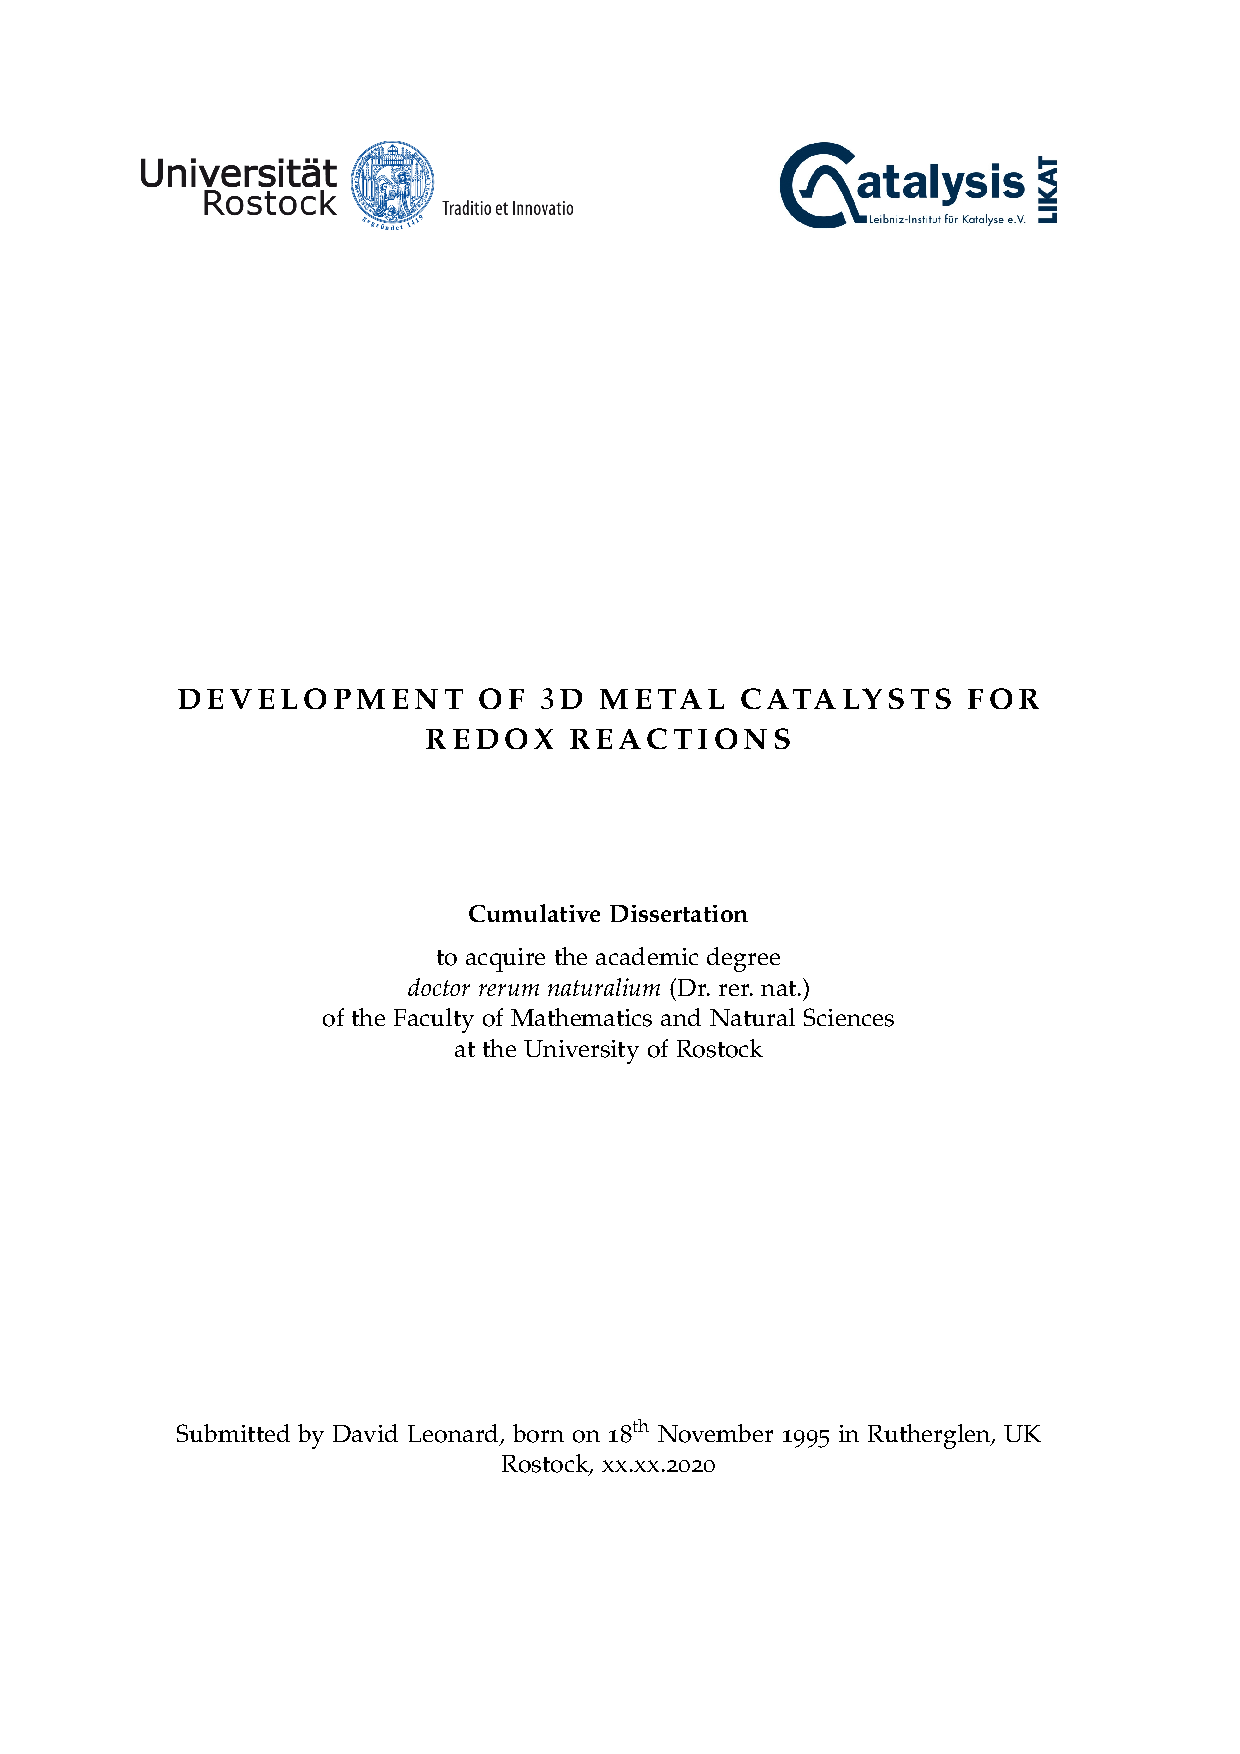
\includepdf[pages=-]{pdf/title.pdf}

\cleardoublepage% Declaration

\refstepcounter{dummy}
\pdfbookmark[0]{Declaration}{declaration} % Bookmark name visible in a PDF viewer

\chapter*{Statement of Authorship} % Declaration section text

\thispagestyle{empty}

\noindent I hereby affirm that I have written the present work by myself without outside assistance. No other resources were utilised than stated. All references as well as verbatim extracts were quoted and all sources of information were specifically acknowledged.\\

\noindent Ich versichere hiermit an Eides statt, dass ich die vorliegende Arbeit selbstst\"andig angefertigt und ohne fremde Hilfe verfasst habe. Dazu habe ich keine au{\ss}er den vin mir angegebenen Hilfsmitteln und Quellen verwendet und die den benutzten Werken inhaltlich und w\"ortlich entnommenen Stellen habe ich als solche kenntlich gemacht.

\
\bigskip
 
\noindent\textit{\myLocation, \myTime}

\smallskip

\begin{flushright}
\begin{tabular}{m{5cm}}
\\ \hline
\centering\myName \\
\end{tabular}
\end{flushright}
 % Declaration

\cleardoublepage% Dedication

\thispagestyle{empty}
\refstepcounter{dummy}

\pdfbookmark[1]{Dedication}{Dedication} % Bookmark name visible in a PDF viewer

\vspace*{3cm}

\begin{center}
%\emph{Ohana} means family. \\
%Family means nobody gets left behind, or forgotten. \\ \medskip
%--- Lilo \& Stitch    
\end{center}

\medskip

\begin{center}
%Dedicated to the loving memory of Rudolf Miede. \\ \smallskip
%1939\,--\,2005

Dedicated to the loving memory of my grandfather,\\ \textbf{George Laurenson Docharty} \\ \smallskip
1930\,--\,2020
\end{center}
 % Dedication page

%\cleardoublepage\include{FrontBackMatter/Foreword} % Uncomment and create a Foreword.tex to include a foreword

\cleardoublepage% Abstract

%\renewcommand{\abstractname}{Abstract} % Uncomment to change the name of the abstract

\pdfbookmark[1]{Abstract}{Abstract} % Bookmark name visible in a PDF viewer

\begingroup
\let\clearpage\relax
\let\cleardoublepage\relax
\let\cleardoublepage\relax

\chapter*{Abstract}
% Short summary of the contents\dots a great guide by 
% Kent Beck how to write good abstracts can be found here:  
% \begin{center}
% \url{https://plg.uwaterloo.ca/~migod/research/beckOOPSLA.html}
% \end{center}

Catalytic methods for the site-selective scission of C(sp$^{3}$)--C(sp$^{3}$) bonds remain scarcely explored in contrast to the vist literature on C--C coupling. In view of this, we report a means of oxidative C--C single-bond cleavage in morpholines, made possible by a synergy between cobalt and manganese catalysts using air as a benign oxidant. We demonstrate the synthesic utility of this system with the late-stage oxidative cleavage of Linezolid.

\endgroup			

\vfill
 % Abstract page

\cleardoublepage% Publications - a page listing research articles written using content in the thesis

\pdfbookmark[1]{Publications}{Publications} % Bookmark name visible in a PDF viewer

\chapter*{Publications} % Publications page text

Some ideas and figures have appeared previously in the following publications:\\

%\noindent Put your publications from the thesis here. The packages \texttt{multibib} or \texttt{bibtopic} etc. can be used to handle multiple different bibliographies in your document.

%\begin{refsection}[ownpubs]
%    \small
%    \nocite{*} % is local to to the enclosing refsection
%    \printbibliography[heading=none]
%\end{refsection}

\begin{enumerate}
    \item Leonard, D. K., Li, W., Junge, K., Beller, M. Improved Bimetallic Cobalt--Manganese Catalysts for Selective Oxidative Cleavage of Morpholine Derivatives. \textit{ACS Catal.} \textbf{2019}, 9, 11125--11129.
    \item Li, W., Liu, W., Leonard, D. K., Rabeah, J., Br\"uckner, A., Junge, K., Beller, M. Practical Catalytic Cleavage of C(sp$^3$)--C(sp$^3$) Bonds in Amines. \textit{Angew. Chem., Int. Ed.} \textbf{2019}, 58, 10693--10697.
\end{enumerate}

%\emph{Attention}: This requires a separate run of \texttt{bibtex} for your \texttt{refsection}, \eg, \texttt{ClassicThesis1-blx} for this file. You might also use \texttt{biber} as the backend for \texttt{biblatex}. See also \url{http://tex.stackexchange.com/questions/128196/problem-with-refsection}.
 % Publications from the thesis page

\cleardoublepage% Acknowledgements

\pdfbookmark[1]{Acknowledgements}{Acknowledgements} % Bookmark name visible in a PDF viewer

%\begin{flushright}{\slshape    
%We have seen that computer programming is an art, \\ 
%because it applies accumulated knowledge to the world, \\ 
%because it requires skill and ingenuity, and especially \\
%because it produces objects of beauty.} \\ \medskip
%--- \defcitealias{knuth:1974}{Donald E. Knuth}\citetalias{knuth:1974} \citep{knuth:1974}
%\end{flushright}

%\bigskip


\begin{flushright}{\slshape    
Dare to be honest and fear no labour.} \\ \medskip
--- Rabbie Burns
%--- \defcitealias{knuth:1974}{Donald E. Knuth}\citetalias{knuth:1974} \citep{knuth:1974}
\end{flushright}

%\bigskip

%----------------------------------------------------------------------------------------

\begingroup

\let\clearpage\relax
\let\cleardoublepage\relax
\let\cleardoublepage\relax

\chapter*{Acknowledgements}

%\noindent Put your acknowledgements here.\\

\noindent First...\noindent

\bigskip

%\noindent\emph{Regarding \mLyX}: The \mLyX\ port was initially done by
%\emph{Nicholas Mariette} in March 2009 and continued by
%\emph{Ivo Pletikosi\'c} in 2011. Thank you very much for your work and the contributions to the original style.

\endgroup
 % Acknowledgements page

\cleardoublepage% Summary

\pdfbookmark[1]{Summary}{Summary} % Bookmark name visible in a PDF viewer

%\begin{flushright}{\slshape    
%We have seen that computer programming is an art, \\ 
%because it applies accumulated knowledge to the world, \\ 
%because it requires skill and ingenuity, and especially \\
%because it produces objects of beauty.} \\ \medskip
%--- \defcitealias{knuth:1974}{Donald E. Knuth}\citetalias{knuth:1974} \citep{knuth:1974}
%\end{flushright}

%\bigskip



%\bigskip

%----------------------------------------------------------------------------------------

\begingroup

\let\clearpage\relax
\let\cleardoublepage\relax
\let\cleardoublepage\relax

\chapter*{Summary}


\noindent Summary here...

%\noindent\emph{Regarding \mLyX}: The \mLyX\ port was initially done by
%\emph{Nicholas Mariette} in March 2009 and continued by
%\emph{Ivo Pletikosi\'c} in 2011. Thank you very much for your work and the contributions to the original style.

\endgroup
 % Summary page

\cleardoublepage% Summary

\pdfbookmark[1]{List of Abbreviations}{List of Abbreviations} % Bookmark name visible in a PDF viewer

%\begin{flushright}{\slshape    
%We have seen that computer programming is an art, \\ 
%because it applies accumulated knowledge to the world, \\ 
%because it requires skill and ingenuity, and especially \\
%because it produces objects of beauty.} \\ \medskip
%--- \defcitealias{knuth:1974}{Donald E. Knuth}\citetalias{knuth:1974} \citep{knuth:1974}
%\end{flushright}

%\bigskip



%\bigskip

%----------------------------------------------------------------------------------------

\begingroup

\let\clearpage\relax
\let\cleardoublepage\relax
\let\cleardoublepage\relax

\chapter*{List of Abbreviations}

\begin{table}[ht]
\centering
\begin{tabular}{ l l }
\toprule
$\delta$ & chemical shift \\
equiv & equivalents \\
Et & ethyl \\
\textit{J} & coupling constant \\
Me & methyl \\
NMR & nuclear magnetic resonance \\
ppm & parts per million \\
TEMPO & $2$,$2$,$6$,$6$-tetramethylpiperidinyloxyl \\
TMS & trimethylsilane \\
\bottomrule
\end{tabular}
\label{tab:SI}
\end{table}

%\noindent\emph{Regarding \mLyX}: The \mLyX\ port was initially done by
%\emph{Nicholas Mariette} in March 2009 and continued by
%\emph{Ivo Pletikosi\'c} in 2011. Thank you very much for your work and the contributions to the original style.

\endgroup
 % Abbreviations page

\cleardoublepage% Summary

\pdfbookmark[1]{Units of Measurement}{Units of Measurement} % Bookmark name visible in a PDF viewer

%\begin{flushright}{\slshape    
%We have seen that computer programming is an art, \\ 
%because it applies accumulated knowledge to the world, \\ 
%because it requires skill and ingenuity, and especially \\
%because it produces objects of beauty.} \\ \medskip
%--- \defcitealias{knuth:1974}{Donald E. Knuth}\citetalias{knuth:1974} \citep{knuth:1974}
%\end{flushright}

%\bigskip



%\bigskip

%----------------------------------------------------------------------------------------

\begingroup

\let\clearpage\relax
\let\cleardoublepage\relax
\let\cleardoublepage\relax

\chapter*{Units of Measurement}


\noindent The International System of Units (SI) is utilised throughout this work to measure experimental of theoretical quantities. All derived units and their expression in terms of the SI bas units are given below.\bigskip

\begin{table}[h!]
\centering
\begin{tabular}{ l l l l }
\toprule
quantity & unit & name & conversion to SI base units \\
\midrule
temperature & $^{\circ}$C & degrees celsius &T/K$=$T/$^{\circ}$C$-273.15$ \\
volume & mL & millilitre & $1$ mL = $1$ cm$^3$ = $10^{-6}$ m$^3$ \\
\bottomrule
\end{tabular}
\label{tab:SI}
\end{table}

%\noindent\emph{Regarding \mLyX}: The \mLyX\ port was initially done by
%\emph{Nicholas Mariette} in March 2009 and continued by
%\emph{Ivo Pletikosi\'c} in 2011. Thank you very much for your work and the contributions to the original style.

\endgroup
 % Units of Measurement page

\pagestyle{scrheadings} % Show chapter titles as headings

\cleardoublepage% Table of Contents - List of Tables/Figures/Listings and Acronyms

\refstepcounter{dummy}

\pdfbookmark[1]{\contentsname}{tableofcontents} % Bookmark name visible in a PDF viewer

\setcounter{tocdepth}{2} % Depth of sections to include in the table of contents - currently up to subsections

\setcounter{secnumdepth}{3} % Depth of sections to number in the text itself - currently up to subsubsections

\manualmark
\markboth{\spacedlowsmallcaps{\contentsname}}{\spacedlowsmallcaps{\contentsname}}
\tableofcontents 
\automark[section]{chapter}
\renewcommand{\chaptermark}[1]{\markboth{\spacedlowsmallcaps{#1}}{\spacedlowsmallcaps{#1}}}
\renewcommand{\sectionmark}[1]{\markright{\thesection\enspace\spacedlowsmallcaps{#1}}}

\clearpage

\begingroup 
\let\clearpage\relax
\let\cleardoublepage\relax
\let\cleardoublepage\relax

%----------------------------------------------------------------------------------------
%	List of Figures
%----------------------------------------------------------------------------------------

\refstepcounter{dummy}
%\addcontentsline{toc}{chapter}{\listfigurename} % Uncomment if you would like the list of figures to appear in the table of contents
\pdfbookmark[1]{\listfigurename}{lof} % Bookmark name visible in a PDF viewer

\listoffigures

\vspace{8ex}
\newpage

%----------------------------------------------------------------------------------------
%	List of Tables
%----------------------------------------------------------------------------------------

\refstepcounter{dummy}
%\addcontentsline{toc}{chapter}{\listtablename} % Uncomment if you would like the list of tables to appear in the table of contents
\pdfbookmark[1]{\listtablename}{lot} % Bookmark name visible in a PDF viewer

\listoftables
        
\vspace{8ex}
\newpage
    
%----------------------------------------------------------------------------------------
%	List of Listings
%---------------------------------------------------------------------------------------- 

\refstepcounter{dummy}
%\addcontentsline{toc}{chapter}{\lstlistlistingname} % Uncomment if you would like the list of listings to appear in the table of contents
\pdfbookmark[1]{\lstlistlistingname}{lol} % Bookmark name visible in a PDF viewer

\lstlistoflistings 

\vspace{8ex}
\newpage
       
%----------------------------------------------------------------------------------------
%	Acronyms
%----------------------------------------------------------------------------------------

\refstepcounter{dummy}
%\addcontentsline{toc}{chapter}{Acronyms} % Uncomment if you would like the acronyms to appear in the table of contents
\pdfbookmark[1]{Acronyms}{acronyms} % Bookmark name visible in a PDF viewer

\markboth{\spacedlowsmallcaps{Acronyms}}{\spacedlowsmallcaps{Acronyms}}

\chapter*{Acronyms}

\begin{acronym}[UML]
\acro{DRY}{Don't Repeat Yourself}
\acro{API}{Application Programming Interface}
\acro{UML}{Unified Modeling Language}
\end{acronym}  
                   
\endgroup % Contents, list of figures/tables/listings and acronyms

\cleardoublepage

\pagenumbering{arabic} % Arabic page numbering for thesis content (1, 2, 3, etc)
%\setcounter{page}{90} % Uncomment to manually start the page counter at an arbitrary value (for example if you wish to count the pre-content pages in the page count)

\cleardoublepage % Avoids problems with pdfbookmark

%----------------------------------------------------------------------------------------
%	THESIS CONTENT - CHAPTERS
%----------------------------------------------------------------------------------------

\ctparttext{You can put some informational part preamble text here. Illo principalmente su nos. Non message \emph{occidental} angloromanic da. Debitas effortio simplificate sia se, auxiliar summarios da que, se avantiate publicationes via. Pan in terra summarios, capital interlingua se que. Al via multo esser specimen, campo responder que da. Le usate medical addresses pro, europa origine sanctificate nos se.} % Text on the Part 1 page describing  the content in Part 1

%\part{Some Kind of Manual} % First part of the thesis

% Chapter 1

\chapter{Target and Motivation} % Chapter title

\label{ch:target} % For referencing the chapter elsewhere, use \autoref{ch:introduction} 

%----------------------------------------------------------------------------------------

\noindent The cleavage of C(sp$^3$)$-$C(sp$^3$) is arguably one of the most challenging transformations in chemistry and doing so is highly difficult to achieve in a mild and selective manner that is compatible with organic synthetic strategies. C$-$C single bond cleavage reactions are of the utmost importance in the petrochemical industry where crude oil is \textit{cracked} into an assortment of smaller hydrocarbon fractions for further processing and for maximising of value. Whilst these reactions are carried out routinely in the industrial sector using heterogeneous catalysts, the low selectivity and harsh reaction conditions necessitated ($>300$\textsuperscript{$\circ$}C) renders this an unsuitable solution for the synthesis of a diverse range of functionalised organic compounds bearing sensitive chemical motifs.

Homogeneous catalysts generally offer the attractive properties of being both highly active and highly selective (cf. heterogeneous catalysts) whilst allowing more potential for catalyst \textit{tuning} and greater mechanistic insight. In contrast to heterogeneous systems, where reactions take place on non-ideal catalyst surfaces, homogeneous systems typically exist in solution as a single well-defined molecular species with only one available reaction site available, resulting in fewer undesired byproducts.

Currently there are very few literature examples of selective cleavage of C(sp\textsuperscript{3})--C(sp\textsuperscript{3}) bonds under mild reaction conditions. Success in this area may provide the potential for: (i) the synthesis of drug metabolites to enable more rapid selection of viable clinical candidates; (ii) improved energy efficiency and selectivity of fossil fuel cracking; (iii) providing renewable chemical feedstocks via the valorisation of biomass. In this thesis, different protocols for the activation of C(sp$^3$)$-$C(sp$^3$) bonds are presented. In each case, $3$d metals are used as catalysts facilitating the oxidation processes, and molecular oxygen---air, in fact---is used as the sole oxidant.

\sloppy{
Aside from that which is outlined above, other topics evolved which I contributed to. Also included in this thesis, therefore, is the development of a nickel-based heterogeneous catalyst for reductive dehalogenation of aryl halides.
}
 % Chapter 1

\cleardoublepage % Empty page before the start of the next part

%------------------------------------------------

\ctparttext{You can put some informational part preamble text here. Illo principalmente su nos. Non message \emph{occidental} angloromanic da. Debitas effortio simplificate sia se, auxiliar summarios da que, se avantiate publicationes via. Pan in terra summarios, capital interlingua se que. Al via multo esser specimen, campo responder que da. Le usate medical addresses pro, europa origine sanctificate nos se.} % Text on the Part 2 page describing the content in Part 2

% \part{The Showcase} % Second part of the thesis


% Chapter 2

\chapter{Introduction} % Chapter title

\label{ch:introduction} % For referencing the chapter elsewhere, use \autoref{ch:examples} 

%----------------------------------------------------------------------------------------

\subsection{Chemistry and Catalysis}

\label{ss:chemistryandcatalysis}

\noindent The natural science of chemistry owes a great deal its origin of \textit{alchemy}---the ancient practice largely dedicated to the transmutation of matter (namely that of lead to gold), founded on the mystical beliefs in the Philosopher's Stone or the Universal Elixir. Many alchemical methods---including also the knowledge acquired from the purification of metals extracted from mining; the preparation of herb-based medicinal remedies; as well as the creation of jewelery---have led to many of the practical techniques in use today's chemistry labs. In fact, it was not until very recently, around the beginning of the seventeenth century, that chemistry began to emerge as a scientific discipline in the modern sense.\textsuperscript{\cite{greenberg:2007}}

With growing concerns regarding anthropogenic climate change, environmental pollution and the rapid depletion of fossil resources we as chemists have persuasive incentives to ensure that chemistry is carried out efficiently, sustainably and in a way that minimises the output of undesirable by-products. To achieve these goals, catalysis remains a key technology by reducing the waste output and energy required for chemical reactions to occur, whilst enabling reactions which would not be possible in their absence, whilst increasingi product selectivity and yield. Thus it is not surprising that catalysis is considered to be one of the twelve principles of green chemistry.\textsuperscript{\cite{anastas:1998}}

The power of catalysis has been recognised since ancient times and has in fact been utilised for the development and prosperity of mankind at least as far back as the Neolithic Revolution, ca. 12\,500 years ago. This transitional period marked a worldwide shift in many human cultures away from lifestyles revolving around hunting and gathering towards agriculture and settlement, which is more akin to the modern world. This cultural change led to the development of farming practices and led to the preservation of food supplies using microbes and their biological catalysts, known as enzymes.\textsuperscript{\cite{vogel:2019}}

The earliest evidence of enzyme-assisted brewing can be traced back even further to the Neolithic village of Jiahu in China around 7500 \spacedlowsmallcaps{BCE}, where investigators found early evidence of alcoholic beverages.\textsuperscript{\cite{mcgovern:2004}}

The Egyptians---who were well aware of early enzyme-assisted brewing techniques---also utilised microorganisms and malt to produce bread as far back as 2000$-$1200 \spacedlowsmallcaps{BCE}.\textsuperscript{\cite{samuel:1996}}

Of course mankind hasn't limited its enzyme technologies to just bread and beer. Material applications are indispensible and enzymes have proven advantageous here also. Starting from pigeon and/or dog dung it is possible to use the microbacterial enzymes in the softening of leather. As early as 7000$-$3300 \spacedlowsmallcaps{BCE} this was exploited for leather processing for all manner of tools including bags, boats, and shoes.\textsuperscript{\cite{possehl:1996}}

It was much later, in the begining of the twentieth century, that catalysis as a scientific field was established. Nobel prizes have been highlighted many of the most influential discoveries in this era. Friedrich Wilhelm Ostwald, who recieved a Nobel prize in 1907, was the first to identify the role of catalysts as accelerants of reactions without themselves being consumed in the process, as well as defining the principles of chemical equilibria. Paul Sabatier, subsequently won the Nobel prize winner in 1912 for demonstrating the hydrogenation of organic compounds using fine powdered metals---a synthetic method which remains highly relevant in today's synthetic toolbox.\textsuperscript{\cite{beller:2012}}

Undoubtedly, one of the greatest success stories in catalysis is the development of artificial nitrogen fixation, resulting from one of the world's most successful partnerships between the German chemists Fritz Haber and Carl Bosch. Once Haber demonstrated the catalytic generation of ammonia from nitrogen and hydrogen on benchtop scale, Bosch, who worked at \textit{Badische Anilin- und Soda-Fabrik} (BASF), was instrumental in developing the high pressure reaction vessels and scaling up the reaction to a viable industrial process. After rigorous, state-of-the-art experimentation, an iron catalyst developed by Mittasch,\textsuperscript{\cite{honkala:2005}} was successfully implemented for the generation of ammonia. The process, known now as the Haber--Bosch process, has facilitated the production of inorganic fertilisers and we no longer rely solely on \textit{Rhizobium} bacteria for biofixation of the nitrogen our bodies need to synthesise vital proteins. Ultimately this advancement led to a population boom in the twentieth century from just 1.6 billion in the year 1900 to six billion in 1999.\textsuperscript{\cite{smil:1999}} In fact some estimations indicate that more than half of the world's agricultural yield relies on the Haber--Bosch process, which continues to feed the world's growing population. The scientific community recognised the advancement by bestowing of two separate Nobel prizes in 1918 and 1931, to Haber and Bosch (with F. Bergius), respectively. 

In 1963, the Nobel prize in chemistry was awarded to Karl Ziegler and Giulio Natta for their chemical and technological discoveries which enable high polymers to be generated from $1$-alkene monomers. A plethora of highly versatile Ziegler--Natta catalysts have been used since the inception of the so-called first-generation in the early 1950s.\textsuperscript{\cite{nowlin:2010}} The industrial value of these findings have been tremendous and has led to the generation of some of the largest volume commodity chemicals on the planet. 

The 1970s saw the development in palladium-mediated cross-coupling reactions and in 2010 the Nobel prize in chemistry was shared between Richard F. Heck, Ei-Ichi Negishi, and Akira Suzuki \textit{for palladium-catalyzed cross couplings in organic synthesis}.\textsuperscript{\cite{nobel:2010}} Nowadays, the Suzuki--Miyaura reaction is the gold standard in biaryl coupling using homogeneous catalysis, and it has become ubiquitous in both academia and industry.

%a new field of chemistry was established, known as catalysis. Catalysis is a relatively new as a scientific discipline established its roots at the beginning of the twentieth century. Already for many years it was known that the addition of small quantities of a substance to a reaction mixture could vastly improve reaction rates and selctivities without itself being consumed in the process.\textsuperscript{\cite{beller:2012}}

% \noindent Growing concerns regarding anthropogenic climate change, environmental pollution and the rapid depletion of fossil resources are all powerful and persuasive incentives to ensure that chemistry is carried out efficiently, sustainably and in a way that minimises the output of undesirable by-products. Naturally, catalysis remains a key technology in this respect, by reducing the waste output and energy required for chemical reactions to occur, whilst enabling reactions which would not be possible in their absence, whilst increasingi product selectivity and yield. Thus it is not surprising that catalysis is considered to be one of the twelve principles of green chemistry.\textsuperscript{\cite{anastas:1998}}

Over time the very definition of a catalyst has evolved as our understanding of them has grown, but nowadays a catalyst is considered: \textit{a substance that increases the rate of a reaction without modifying the overall standard Gibbs energy change in the reaction}.\textsuperscript{\cite{iupac:2014}}

Catalysts by their very nature reduce the activation barrier (\textit{E}\textsubscript{a}) required for a reaction to occur and this is achieved by providing an alternative mechanism for the reactants to follow.

Nowadays ca. 85\% of all industrial chemical processes involve at least one catalytic step. This is a reflection of their abilities in accelerating transformations, promoting selectivity, and reducing waste output and energy consumption. Whilst for many decades rare and precious second and third row transition metals have been at the forefront of catalysis, today's state-of-the-art catalysts are increasingly dependent on the talents of Earth-abundant 3d-metals.\textsuperscript{\cite{hapke:2020}}

\subsection{Homogeneous vs. Heterogeneous Catalysis}

Catalysts can be divided into two main categories: \textit{homogeneous} catalysts and \textit{heterogeneous} catalysts. The main distinction is the relative physical states of the catalyst and the reacion mixture; in homogeneous catalysis the catalyst is in the same phase as the rest of the reaction mixture, whereas in heterogeneous catalysis the catalyst is in a different phase from the rest of the reaction mixture. In most cases a homogeneous catalyst is dissolved in a solution of reagents, and a heterogeneous catalyst is a solid which is insoluble in solution.

Both classes of catalysts have their advantages and disadvantages (summarised in Table \ref{tab:comparison}).

Heterogeneous catalysts are widely utilised in the chemical industry than homogeneous catalysts. One of the main reasons for this is the ease of separation of the catalyst (normally a solid) from reaction mixtures.

\begin{table}[h!]
\centering
\caption[General Differences Between Homogeneous and Heterogeneous Catalysts]{General Differences Between Homogeneous and Heterogeneous Catalysts}
\begin{tabular}{ c c }
\toprule
homogeneous & heterogeneous \\
\midrule
 well-defined active site & many possible active sites \\
 high selectivity & low selectivity \\
 difficult separation & facile separation \\
 react at low temperature & react at high temperature \\
\bottomrule
\end{tabular}
\label{tab:comparison}
\end{table}

\section{Copper}

Copper, with the symbol Cu and atomic number $29$ is positioned in the the $3$d-block of the periodic table between nickel and zinc. It is a naturally occuring trace element (\ie\, comprises $<0.1$ mg kg$^{-1}$ of the earth's crust) found in rocks and minerals and plays an important biochemical role as an essential micronutrient and for facilitating metabolic processes in both prokaryotes and eukaryotes.\textsuperscript{\cite{flemming:1989}}

Copper's capabilities in redox catalysis are well documented, and is widely utilised in nature in the metal centres of at least $25$ biological enzymes. Myriad oxidation processes are facilitated by copper-containing enzymes, including: cytochrome c oxidase, superoxide dismutase, amine oxidase, lysyl oxidase, dopamine $\beta$-hydroxylase, peptidylglycine $\alpha$-amidating monooxygenase, tyronsinase, galactose oxidase, hemocyanin, ceruloplasmin, laccase, and acorbate oxidase. What's more, each of these enzymes relies on molecular oxygen as the oxidant.\textsuperscript{\cite{tishchenko:2016}}

\section{Manganese}

Manganese, with the symbol Mn and atomic number 25, is positioned in the the 3d-block of the Periodic table between chromium and iron. It is the twelfth most abundant element in the Earth's crust,\textsuperscript{\cite{costa:2014}} and it's known for its remarkable ability to exist in many oxidation states which range from $-3$ to $+7$, of which $+2$, $+3$, $+4$, $+6$, and $+7$ are most common.

Mn was not recognised as an element until 1774 when German$-$Swedish chemist, Carl Wilhelm Scheele, analysed pyrolusite (MnO$_2$) and recognised the that the ore and its extracts contained a previously undiscovered element! However, it wasn't until Scheele supplied Johan Gottlieb Gahn, a Swedish chemist and metallurgist, with pyrolusite that elemental manganese was first extracted later that year.\textsuperscript{\cite{kemmitt:1973}} 

Despite appearing silver$-$grey in its pure metallic form, given its propensity towards oxidation, it's found in Nature in oxidised forms, such as the ores pyrolusite, romanechite, manganite, hausmannite, and rhodochrosite, etc. 

Mn is an element essential for all life on Earth and it takes an active role in metabolism of amino acids, lipids, proteins and carbohydrates. In fact it's encountered in myriad animal systems, including those responsible for immunity, reproduction, blood sugar regulation, and bone growth.\textsuperscript{\cite{banci:2012}}

Plants also rely on Mn to facilitate photosynthesis---the process which generates the very oxygen we breathe---by forming the metalloenzyme core within the chloroplasts.\textsuperscript{\cite{banci:2012}}

Despite its ubiquity in terrestrial life, some guidance regarding limits of consumption of Mn are given by the U.\,S. National Research Council (NRC); It has provided an \textit{\textbf{e}stimated \textbf{s}afe and \textbf{ad}equate \textbf{d}ietary \textbf{i}ntake} (ESADDI), which recommends adults consume between 2$-$5 mg day$^{-1}$ of Mn.\textsuperscript{\cite{banci:2012}}

In fact, overexposure to Mn can be highly damaging towards human health. Manganism (Mn poisoning) was first observed in 1837 by James Couper, who documented the neurological damage of five Scottish men who were suffering after grinding manganese dioxide. Chronic exposure to Mn only proliferated therafter as Mn became increasingly ubiquitary in the steel alloy industry. Fortunately, exposure to the levels of Mn detailed by Couper are rare. Nevertheless, concerns regarding its impact on human health are valid.\textsuperscript{\cite{costa:2014}}

For a comprehensive peer-reviewed toxicological overview, see the U.\,S. Agency for Toxic Substances and Disease Registry's 2012 report.\textsuperscript{\cite{williams:2012}} Therein the authors quote \textit{adequate intakes} of 2.3 mg day$^{-1}$ and 1.8 mg day$^{-1}$ for men and women, respectively, based on data sourced from the U.\,S. Institute of Medicine Food and Nutrition Board.\textsuperscript{\cite{trumbo:2001}}

\section{Iron}

Iron, with the symbol Fe and atomic number $26$ is positioned in the the $3$d-block of the Mendeleev table between manganese and cobalt. Despite being the most abundandant element on Earth (by mass), it constitutes just ca. $5$\% of the Earth's crust, making it the the fourth most abundant element therein.\textsuperscript{\cite{nicholls:1973}}

Metallic iron is rarely found in the earth's crust, occuring much almost always in an oxidised form, and thus mankind has been extracting Fe from ores as far back as ca. $1200$ \spacedlowsmallcaps{BCE}. Oxides and carbonates, such as \textit{magnetite} (Fe$_3$O$_4$), \textit{hematite} (Fe$_2$O$_3$) and \textit{siderite} (FeCO$_3$), constitute the most common ores of iron. Besides those, are sulfur- and silicate-based ores, including \textit{pyrite} (FeS$_2$) and \textit{silicate perovskite} (FeSiO).\textsuperscript{\cite{nicholls:1973}}

Iron is ferromagnetic, and has a Curie point (the temperature at which certain magnetic materials undergo a sharp change in their magnetic properties) of $768^{\circ}$C, at which point it undergoes an endothermic transformation to its paramagnetic form.\textsuperscript{\cite{nicholls:1973}} From the perspective of catalysis, iron has properties which make it a distinguished adversary in the field of homogeneous catalysis. Iron has a wide breadth of formal oxidation states which range from $-2$ to $+6$.\textsuperscript{\cite{fuerstner:2016}}

Biologically speaking, iron is an essential element for much of the animal life on Earth, playing an important role in the blood of most vertebrates. It binds readily with porphyrin-derived ligands to form, most notably, the oxygen-transport metalloproteins haemoglobin and myoglobin.

Iron has been used extensively in organometallic chemistry and catalysis. Famously it was utilised by German--Jewish chemist, Peter Pauson, and his student, Thomas J. Kealy, to create \textit{ferrocene}---the first known sandwich complex. Regrettably, both failed to identify the correct structure of the complex, and it wasn't until $1952$ that three groups (including Robert Burns Woodward) independently deduced the correct $\eta^{5}$ hapticity of the iron metallocene.

\section{Cobalt}

Cobalt, with the symbol Co and atomic number 27, is positioned in the 3d-block of the Mendeleev table between iron and nickel. It derived its name in medieval times from the German word \textit{Kobold} meaning Goblin, due to its resemblance to the more sought-after silver$-$copper ores mined in this era, but wasn't recognised as a discrete element until 1735 by Swedish chemist Georg Brand.

Cobalt has a d\textsuperscript{9} electron configuration and readily achieves formal oxidation states ranging from $-$1 to $+$3. In catalytic transformations it has a clear tendency towards the $+$1/$+$3 oxidation states, much like its noble neighbours, rhodium and iridium.\textsuperscript{\cite{hapke:2020}}

The demand for cobalt is intense in today's technological society as consumers rely increasingly on devices integrating rechargable batteries, including mobile phones, laptops, and increasingly, electric vehicles.\textsuperscript{\cite{crundwell:2011}}

The copper$-$cobalt mines in the Central Africa Copperbelt in the Democratic Republic of the Congo (DRC) (such as the much-publicised Mutanda Mine, shown in figure \ref{fig:mutanda}) and Zambia account for more than two thirds of the world's cobalt production, much of which is obtained as a by-product of coper and nickel extraction. It is found in sulfide ores (ca. 25\%), laterite ores (ca. 25\%)...\textsuperscript{\cite{crundwell:2011, wef:2020}}

\begin{figure}
\centering
\begin{minipage}{\textwidth}
   \centering
   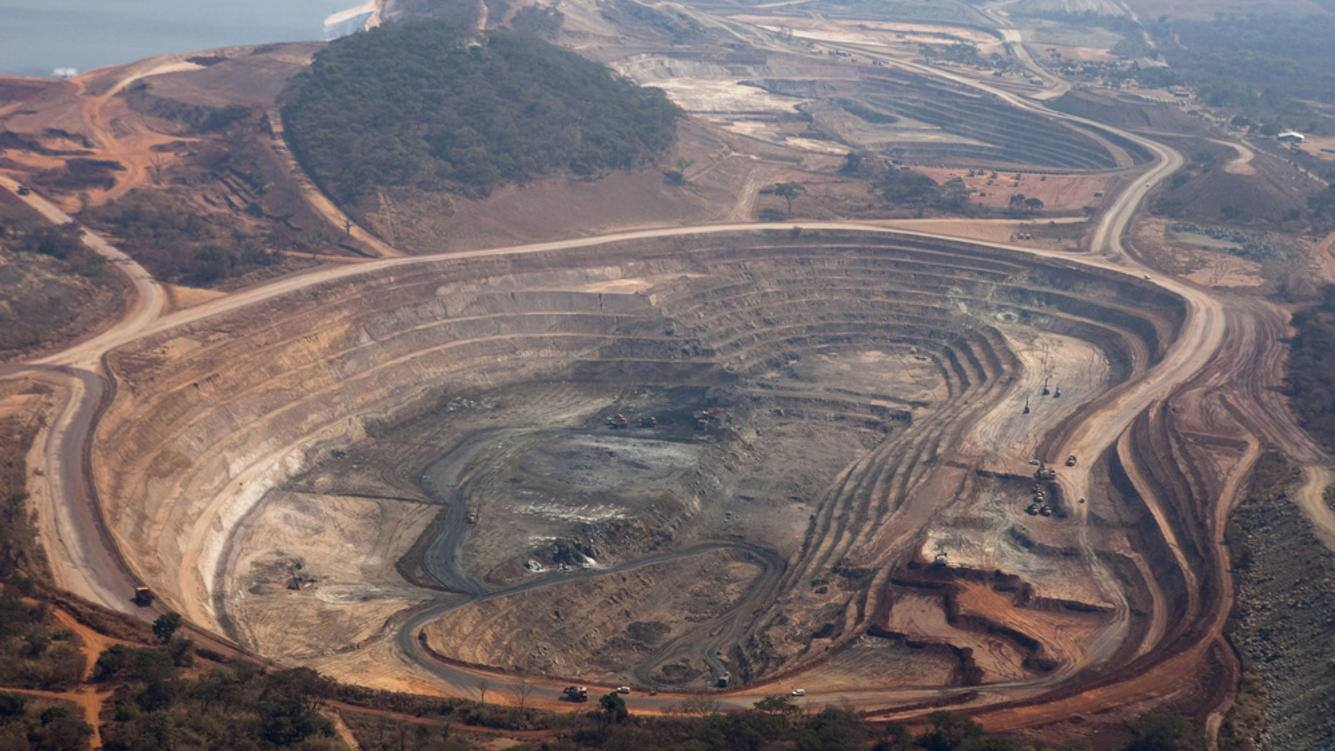
\includegraphics[height=6.5cm]{gfx/mutanda} % figure itself
   \caption{The Mutanda Mine in the DRC. Source: Bloomberg}
   \label{fig:mutanda}
\end{minipage}\hfill
\end{figure}

Cobalt has played an important role in homogeneous catalysis as far back as the 1930s, when the German chemist, Otto Roelen, developed the world's first industrial hydrosilylation process (the \textit{oxo synthesis}) at Oxo Chemie.\textsuperscript{\cite{hapke:2020}}

In biological systems, cobalt is an essential trace element, most notably as an integral component in all four forms of vitamin B$_{12}$.

Notably, the famous Fischer$-$Tropsch process---which converts syngas or watergas into liquid hydrocarbons---relies almost universally on heterogeneous cobalt as the chief catalyst metal and has done so since its inception in 1925. Besides this, presently there are endeavours to further capitalise on the catalytic talents of cobalt for water splitting and CO\textsubscript{2} reduction.\textsuperscript{\cite{wang:2016, gao:2016}}

\section{Oxidations}
  
\noindent Molecular oxygen (O$_2$) is an attractive oxidant for several reasons.\textsuperscript{\cite{gavriilidis:2016}} In production settings, however, oxidations are avoided wherever possible since they are associated with use of toxic metals, halogenated solvents, undesired byproducts and poor atom economy. Therefore, process chemists are severely limited by their choice of possible reagents which must be in the necessary (or higher) oxidation level. From this perspective, molecular oxygen is ideal, given its advantage towards the atom economy of a given oxidation reaction. There are two major chief drawbacks to the adoption of aerobic oxidations in large scale processes, most notably in the pharmaceutical industry: (i) using organic solvents in the presence of oxygen poses a risk to safety, and (ii) their is a lack of efficient catalysts with satisfactory activities and selectivities for such transformations.\textsuperscript{\cite{osterberg:2014}}

In pharmaceutical synthesis organic solvents are often necessary, particularly for ensuring complete solvation of reagents and catalysts, etc. Combining fuel/oxidiser mixtures under heating and increased pressure presents an obvious risk of ignition which is challenging to alleviate.\textsuperscript{\cite{lewis:1987}} Whilst there have been industry-sponsored studies on the flammability of organic solvent vapours,\textsuperscript{\cite{brooks:2007, zabetakis:1965}} there is a distinct lack of data on the safe operation of aerobic oxidations at temperatures and pressures conducive for pharmaceutical processes.\textsuperscript{\cite{osterberg:2014}}

The Amoco process (named after the now-defunct \textbf{Am}erican \textbf{O}il \textbf{Co}mpany) represents a catalytic success story for oxidation chemistry and catalysis. The process is the predominant method of generating terphthalic acid, which is an industrially significant precursor for condensation polymers, such as polyethylene terephthalate. Interestingly, the autooxidation of \textit{para}-xylene to terephthalic acid relies on a unique combination of two homogeneous catalysts and an additional bromide source, which acts as a promoter. The Co$-$Mn$-$Br catalyst system is very much the key to the success of the process, which introduces new catalyst pathways and increases the catalyst activity by 16 times, compared to a single cobalt catalyst.\textsuperscript{\cite{tomas:2013, brill:1960}}

Nitrous oxide (N$_2$O) gas is another attractive oxidant these days. Whereas oxidising with O$_2$ gas may be consumed in a reaction by incorporation into the substrate, N$_2$O gas has the advantage of being itself reduced, forming new---and very stable---N$_2$ gas molecules. Clearly a real benefit can be had over O$_2$ when it comes to achieving a favourable reaction entropy and providing a $-\Delta$G (negative Gibbs free energy change) for any given oxidation.

\section{C$-$C Single Bond Cleavage}

\noindent As mentioned in \autoref{ss:chemistryandcatalysis}, carbon--carbon cross-coupling chemistry has been a focal point in synthetic chemistry since the 1970s. The success of the Suzuki--Miyaura, Kumada, Negishi, Sonogashira, Hiyama, Heck, and Stille reactions are a remarkable testiment to the demand for practical C$-$C bond-forming methodologies, and to modern day chemists C$-$C bond formation is considered a straighforward synthetic strategy for building molecular complexity.

Over the past several decades, the challenge of C--H bond activations has been tackled independently by many groups and has led to many innovative novel publications. Notably, in 1993 Murai et al. reported a highly innovative means of C--H bond functionalisation using catalytic amounts of an organometallic ruthenium complex.\textsuperscript{\cite{murai:1993}} This reaction---considered to be a milestone in contemporary chemistry---demonstrated that the site-selective functionalisation of non-polar $\sigma$-bonds could be both highly practical and atom-economic in the scope of organic synthesis which has since become a well-established field of chemistry.\textsuperscript{\cite{crabtree:2017, labinger:2017, roque:2018}}

In addition to bond forming reactions, bond breaking can offer an alternative means of enhancing structural complexity into organic frameworks in ways that are not easily generated in any other way. Despite their pervasiveness in organic compounds, C$-$C single bond activations remain a real synthetic challenge.

The bond dissociation energy (BDE) of C$-$C, C$=$C, and C$\equiv$C bonds are $347-377$ kJ mol$^{-1}$, $~710$ kJ mol$^{-1}$, and $~960$ kJ mol$^{-1}$, respectively. One would expect, therefore, that C$-$C bonds are far more easily broken than C$=$C and C$\equiv$C bonds.

Oxidative addition of C$-$C bonds is difficult to achieve thermodynamically, as the strength of C$-$C bonds are far stronger than metal--carbon bonds. Substrates are typically more inclined towards C$-$C bond cleavage if they are high in cyclic strain, or if they can gain aromaticity and thus form products low in free energy.\textsuperscript{\cite{sattler:2010, crabtree:2019}} C$-$C single bonds are particularly unreactive when both carbon atoms are sp$^3$ hybridised; such an electron configuration is highly kinetically stable due to a combination of steric hindrance of nearby atoms (\eg, C--H bonds) and the directional nature of the sp\textit{\textsuperscript{n}} hybridised orbitals used in covalent bonding. Furthermore, much of organic synthesis takes advantage of the reactivity of (i) $\pi$-bonds (e.g., C$=$C, C$=$O, etc.), (ii) polarised $\sigma$-bonds (\eg, C--Br, C--Li, etc.), and (iii) lone pairs of electrons.\textsuperscript{\cite{murakami:2016}} Carbon$-$hydrogen and carbon$-$carbon $\sigma$-bonds---which are ubiquitous in the scaffold of organic compounds---are distinctly lacking all three of these basic prerequisites for desireable reactivity.

\begin{figure}
\centering
\begin{minipage}{\textwidth}
   \centering
   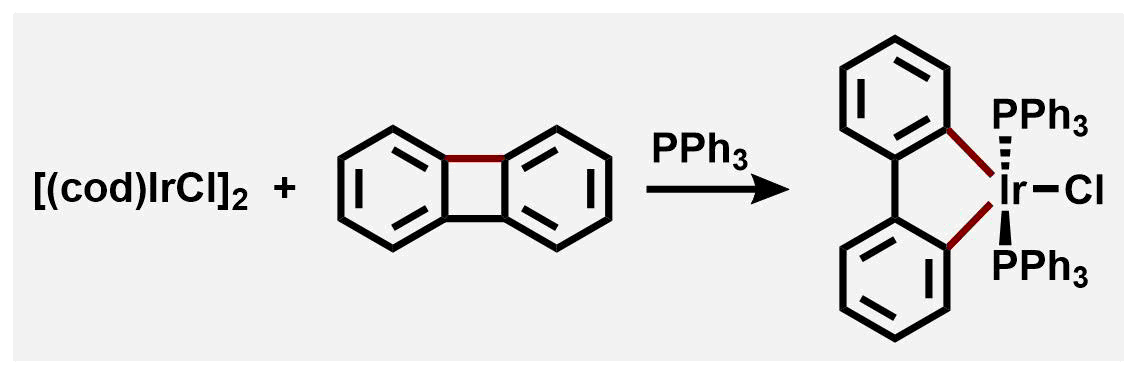
\includegraphics[height=3cm]{gfx/crabtree1} % figure itself
   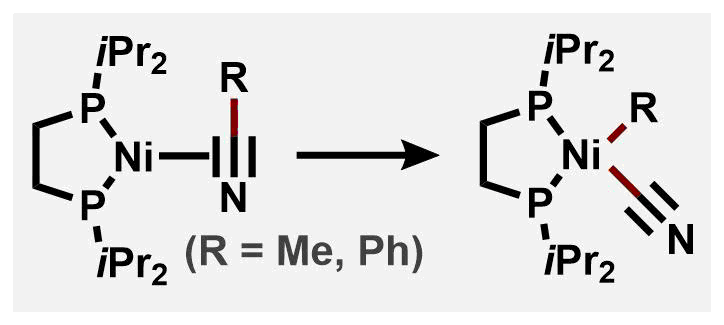
\includegraphics[height=3cm]{gfx/crabtree2} % figure itself
   \caption{Rare examples of C$-$C oxidative additions}
   \label{fig:crabtree}
\end{minipage}\hfill
\end{figure}

%\begin{figure}
%\centering
%\begin{minipage}{\textwidth}
%   \centering
%   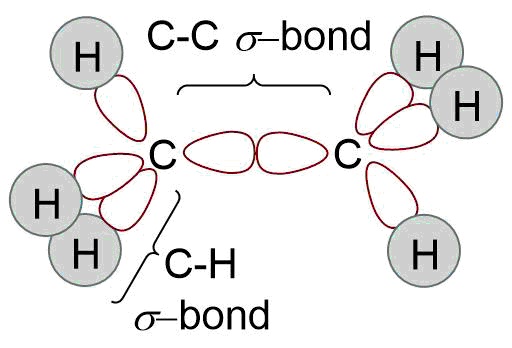
\includegraphics[height=3cm]{gfx/ethane} % figure itself
%   \caption{Ethane molecule: the simplest C(sp\textsuperscript{3})--C(sp\textsuperscript{3}) bond.}
%   \label{fig:ethane}
%\end{minipage}\hfill
%\end{figure}

\subsection{Applications}

C$-$C single bonds are broken routinely in industry where a long-chain hydrocarbon feedstock (such as naphtha) undergoes valorisation inside steam crackers. This energy-intense process is performed at high temperatures ($>$300$^{\circ}$C) to generate lighter hydrocarbons (typically olefins). Likewise, in the organic synthetic laboratory, C$-$C bond cleavage is well-documented using (over)-stoichiometric oxidants. Typical reagents include O$_3$,\textsuperscript{\cite{saliu:2012, suarez-bertoa:2012}} NaIO$_4$,\textsuperscript{\cite{binder:2008}} H$_5$IO$_6$, Pb(OAc)$_4$,\textsuperscript{\cite{criegee:1931}} and KMnO$_4$.

At the heart of many large chemical manufacturing plants is the steam cracker. This crucial piece of process technology provides the starting point for a value chains by taking crude oil fractions (typically naphtha) and "cracking" long chain saturated hydrocarbons into smaller unsaturated compounds, such as ethene and propene; these are the building blocks for myriad chemical comodities. The process for the cleavage of large hydrocarbons is facilitated by a heterogeneous catalyst---often zeolite-based---at temperatures of around 850$^{\circ}$C.

\subsection{Traditional Methods}

\noindent In 1931 Rudolf Criegee and co-workers first reported the cleavage of C(sp$^3$)$-$C(sp$^3$) bonds in vicinal diols (glycols), utilising Pb(OAc)$_4$ as an oxidant to generate aldehyde C(sp$^2$) centres on the two fragments.\textsuperscript{\cite{criegee:1931}} The Criegee oxidation works most effectively with diols glycols with hydroxy groups in close proximity.  \textit{cis}- and \textit{trans}-substituted diols may both proceed by forming a 5-membered cyclic intermediate with the lead atom. In the case of \textit{trans} substrates, a higher energy intermediate must be formed due to the relative orientation of the two oxygen atoms and high ring strain. The corresponding \textit{cis} intermediates are generated much more easily and more rapidly, therefore the reaction exhibits much greater selectivity towards \textit{cis} glycols. If the adoption of a highly strained 5-membered intermediate cannot be achieved, an alternative, slower, pathway is available.

In 1934 L\'eon Malaprade similarly reported a method for oxidative cleavage of C(sp$^3$)$-$C(sp$^3$) bonds in glycols but using hypervalent iodine reagent HIO$_4$ as an oxidant.\textsuperscript{\cite{malaprade:1934}} Due to the strong oxidising nature of HIO$_4$ the reaction may be viewed as less widely applicable that the Criegee oxidation, however, to its credit the Malaprade oxidation additionally provides an effective means of cleaving $\beta$-aminoalcohols.

\begin{figure}[hbt!]
\centering
\begin{minipage}{\textwidth}
   \centering
   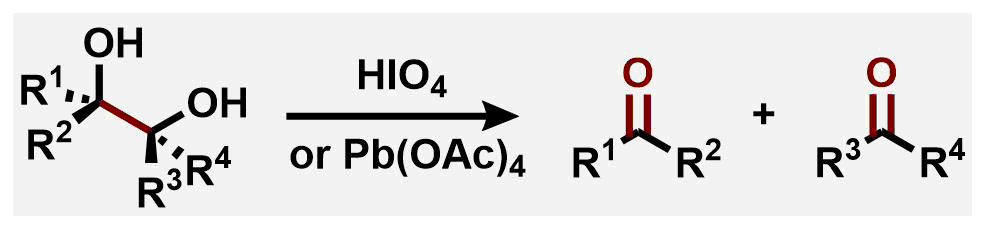
\includegraphics[height=2.2cm]{gfx/malaprade-criegee} % figure itself
   \caption{Criegee and Malaprade oxidations}
   \label{fig:malaprade-malaprade}
\end{minipage}\hfill
\end{figure}

\subsection{State-of-the-Art}

\noindent In recent years there C$-$C single bond activation reactions have come to the attention of chemists as a novel method for introducing valuable complexity within organic compounds. There are comparatively many reports of cleaving C$-$C bonds in there differently hybridised states,\textsuperscript{\cite{zhou:2015, qin:2016, liu:2017, liang:2017, zhao:2018, liu:2019, adeli:2019, tsang:2015}} however the cleavage of C(sp$^3$)$-$C(sp$^3$) bonds is far less reported.

Jiao and co-workers presented in 2017 a novel approach for the oxidative cleavage of allylic C(sp$^3$)$-$C(sp$^3$) bonds in the 

In 2018, Sarpong and co-workers reported a compelling \textit{deconstructive fluorination} methodology, which in a single step, cleaves a C(sp$^3$)$-$C(sp$^3$) bond and incorporates a new C$-$F bond in the process. Selectfluor (4 equiv) is used which acts as a fluorine donor to incorporate valuable complexity into an array of unstrained saturated \textit{N}-heterocycles, as shown in figure \ref{fig:sarpong1}.\textsuperscript{\cite{roque:2018}} Fluorine is widely used in the pharmaceutical and agrochemical industries for its so-called \textit{polar-hydrophobic} nature which can greatly impact lipophility, p\textit{K}\textsubscript{a}, and metabolic stability of small molecules.\textsuperscript{\cite{dalvi:2010}} Whilst this protocol describes the generation of interesting deconstructed products, it does rely on the use of overstoichiometric Selectfluor and AgBF$_4$ (4 equiv of both), and is poorly atom effiecient. Nevertheless, this innovative publication inspired many researchers to investigate the utility of activating C(sp$^3$)$-$C(sp$^3$) bonds for a fundamentally new approach to skeletal diversification. 

\begin{figure}[hbt!]
\centering
\begin{minipage}{\textwidth}
   \centering
   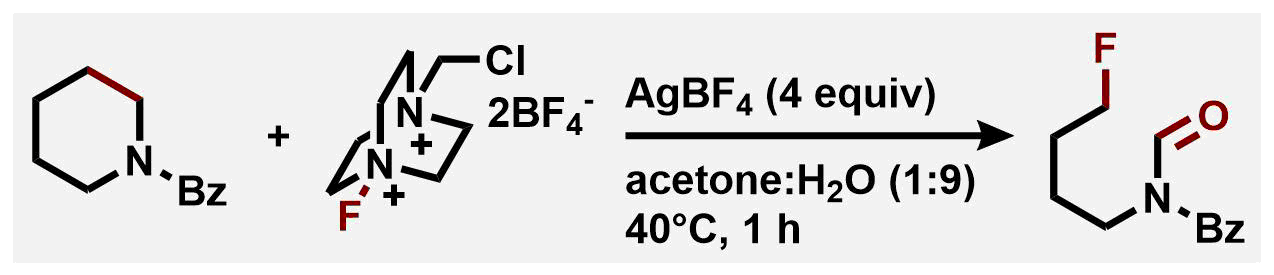
\includegraphics[height=2.5cm]{gfx/sarpong1} % figure itself
   \caption{Deconstructive fluorination using SelectFluor}
   \label{fig:sarpong1}
\end{minipage}\hfill
\end{figure}

The utilisation of lignin in chemistry is highly sought after; it is the main component of lignocellulosic biomass and it is the most ubiquitous renewable source of aromatic units known. Thus it has real potential to be a lucrative feedstock, especially since lignin is a waste product from the paper pulp industry. Phenol, a simple hydroxylated benzene ring, is a valued industrial commodity with a total annual production greater than $11.5$ megatons and is further processed to make dyes, polymers, pharmaceuticals and many other important products.\textsuperscript{\cite{morimoto:2015}} The chemical industry produces phenol from benzene in multistep synthesis under harsh conditions, consuming vast quantities of energy in the process. Naturally, benzene is derived from fossil resources and overall the industrial synthesis of phenol has raised environmental concerns. Achieving selectivity is challenging via this route, given that the hydroxylation of aromatic rings tends towards overoxidation.\textsuperscript{\cite{zhu:2019}} Valorisation of lignin thus presents an interesting, albeit challenging, alternative route towards the synthesis of aromatics such as phenol. Recently, Han and co-workers demonstrated just that, by using a solid acid catalyst and water to facilitate the cleavage of C$-$C single bonds (C(sp$^2$)$-$C(sp$^3$) hybridised) and C$-$O bonds within the complex polymeric material. This procedure was demonstrably effective upon scale-up whereby 4.1 g of phenol was obtained from 50.0 g of lignin.\textsuperscript{\cite{yan:2020}}

\section{Multivariate Optimisation}

\noindent Experimental design is a central concern in academia as well as in industrial chemistry. It is often a challenging endevour to establish fruitful reaction conditions with the optimal combination of reagents, solvents, catalysts, etc. for a reaction.

Univariate optimisation is an investigation of one-factor-at-a-time (OFAT) and is often limited by its small coverage of chemical space and its inability to detect how any interaction between variables may affect the reaction outcomes (\eg, yield, selectivity, etc.).

Reaction optimisation is often performed using a one-factor-at-a-time approach, whereby a scientist only considers a single variable's effect on the outcome of a reaction (\eg\ yield, selectivity, catalyst activity, etc.). Whilst this method can be useful, it is in fact inefficient and often lacking in accuracy. A multivariate analysis of variables on the other hand can be used to investigate a large volume of chemical space in an efficient and expedient manner with greater accuracy than a linear anaysis of variables.

OFAT optimisation rarely provides much insight into which factors are most influencial on the outcome of a reaction and provide no information about any interations between factors which are frequently present.

Design of Experiments (DoE) is a type of multivariate analysis that relies on statistics. In this way, no only can it be used to determine optimal reaction conditions, it also provides the advantage of quantifying the relative effect that each variable has on a reaction outcome. DoE is regularly employed in industry, however it is seldom used in academia despite its many advantages. Its increasingly favourable reputation and popularity amongst industrial chemists is a response to several key reasons:

\begin{enumerate}
  \item The development of high-throughput experimentation (HTE) using parallel reactors and flow reactor setups has become widely implemented.
  \item Quality by testing has largely been superseded by quality by design (QbD) and led to more widespread understanding of design space
  \item Green Chemistry Principles\textsuperscript{\cite{anastas:2010}} have encouraged chemists to reduce the waste output from chemical reactions and increase efficiency by reducing the amounts of solvents and reagents used in chemical processes
\end{enumerate}


Figures \ref{fig:doe-1} and \ref{fig:doe-2} compare the different optimum values obtained from univariate and multivariate analyses, and shows how the order in which factors are investigated will often impact the set of favourable reaction conditions revealed, \ie, the combination of conditions which furnish the most desireable outcome.

\begin{figure}
\centering
\begin{minipage}{0.45\textwidth}
   \centering
   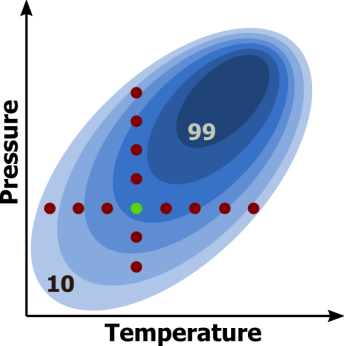
\includegraphics[height=5.4cm]{gfx/doe-1} % first figure itself
   \caption{OFAT study:\\two sequential studies, first exploring T, then \textit{p}}
   \label{fig:doe-1}
\end{minipage}\hfill
\begin{minipage}{0.45\textwidth}
   \centering
   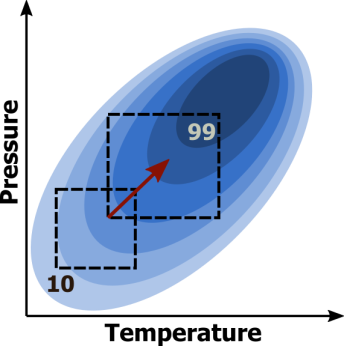
\includegraphics[height=5.4cm]{gfx/doe-2} % second figure itself
   \caption{Full-factorial study:\\one study exploring T and \textit{p} at the same time}
   \label{fig:doe-2}
\end{minipage}
\end{figure}

DoE can be used to investigate the effects of variables at several different numerical values. For this reason, for an effective DoE, it is valuable to have some prior knowledge about the reaction under investigation to select a suitable range of conditions to explore; if all reactions reach zero conversion then it is difficult to ascertain which factors are impeding the progress of the reaction. In other words, one should have at least a vague idea of suitable chemical space to explore.

The most common type of DoE is a \textit{factorial design}, which is represented as a \textit{base} raised to a \textit{power}. The \textit{number of levels} is given by the base, and the \textit{number of variables} is given by the power. Thus a $2^3$ design signifies a two-level three-factorial design. A design of this kind would therefore consist of $8$ experimental runs in addition to, perhaps, $4$ \textit{centre points}---additional experimental runs which are perfromed using the conditions in the very centre of the design space and allow for the reproducability of a reaction to be assessed, and provide a further data point in the optimisation---for a total of $12$ runs. In figure \ref{fig:doe-4} such a design is shown.

As the number of investigation varaiables increases, the number of experimental runs grows exponentially. For large numbers of variables this can be exceptionally demanding not only in terms of the cost of materials and equipment, but also with respect to time. 

\begin{figure}
\centering
\begin{minipage}{0.3\textwidth}
   \centering
   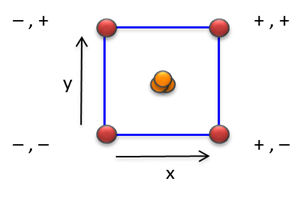
\includegraphics[height=3.2cm]{gfx/doe-3} % first figure itself
   \caption{$2^2$ design}
   \label{fig:doe-3}
\end{minipage}\hfill
\begin{minipage}{0.3\textwidth}
   \centering
   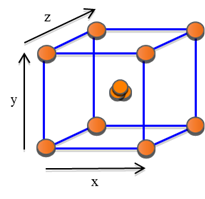
\includegraphics[height=3.2cm]{gfx/doe-4} % second figure itself
   \caption{$2^3$ design}
   \label{fig:doe-4}
\end{minipage}\hfill
\begin{minipage}{0.3\textwidth}
   \centering
   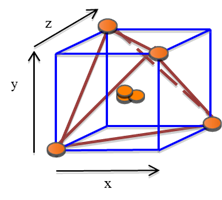
\includegraphics[height=3.2cm]{gfx/doe-5} % second figure itself
   \caption{$2^{3-1}$ design}
   \label{fig:doe-5}
\end{minipage}
\end{figure}

In 2002, Trevor Laird, at the time the editor of \textit{Organic Process Research \& Development} expressed his concerns regarding the reluctance of organic chemists to incorporate DoE techniques in their research, despite their efficacy in areas such as optimisation and for examining structure--activity relationships.\textsuperscript{\cite{laird:2002}}

% Papers to read: weissman:2015
% Diagram of univariate vs. multivariate
DoE has proven effective and gained popularity in industry as a practical tool for reaction optimisation and process improvements. This has been demonstrated by Pfizer with the simplified and cleaner synthesis of sertraline hydrochloride (Zoloft), a popular selective serotonin reuptake inhibitor, used to treat depression and anxiety-related disorders.\textsuperscript{\cite{taber:2004}}
 % Chapter 2
\include{Chapters/Chapter03} % Chapter 3

% Bibliography

\label{app:bibliography} % Reference the bibliography elsewhere with \autoref{app:bibliography}

\manualmark % Work-around to have small caps also here in the headline
\markboth{\spacedlowsmallcaps{\bibname}}{\spacedlowsmallcaps{\bibname}} % Work-around to have small caps also
%\phantomsection
\refstepcounter{dummy}

\addtocontents{toc}{\protect\vspace{\beforebibskip}} % Place the bibliography slightly below the rest of the document content in the table of contents
\addcontentsline{toc}{chapter}{\tocEntry{\bibname}}

\printbibliography % Bibliography

\include{Chapters/Chapter04} % Chapter 4
\include{Chapters/Chapter05} % Chapter 5
%\include{Chapters/Chapter06} % Chapter 6 

\cleardoublepage % Empty page before the start of the next part

%----------------------------------------------------------------------------------------
%	THESIS CONTENT - APPENDICES
%----------------------------------------------------------------------------------------

\appendix

%\part{Appendix} % New part of the thesis for the appendix

\include{Chapters/Chapter0A} % Appendix A
%% Appendix X

\chapter{Appendix Title}

%----------------------------------------------------------------------------------------

% Content begins here
 % Appendix B - empty template

%----------------------------------------------------------------------------------------
%	POST-CONTENT THESIS PAGES
%----------------------------------------------------------------------------------------

%\cleardoublepage% Bibliography

\label{app:bibliography} % Reference the bibliography elsewhere with \autoref{app:bibliography}

\manualmark % Work-around to have small caps also here in the headline
\markboth{\spacedlowsmallcaps{\bibname}}{\spacedlowsmallcaps{\bibname}} % Work-around to have small caps also
%\phantomsection
\refstepcounter{dummy}

\addtocontents{toc}{\protect\vspace{\beforebibskip}} % Place the bibliography slightly below the rest of the document content in the table of contents
\addcontentsline{toc}{chapter}{\tocEntry{\bibname}}

\printbibliography % Bibliography

%\cleardoublepage% Colophon (a brief description of publication or production notes relevant to the edition)

\pagestyle{empty}

\hfill

\vfill

\pdfbookmark[0]{Colophon}{colophon}

\section*{Colophon}

This document was typeset using the typographical look-and-feel \texttt{classicthesis} developed by Andr\'e Miede. The style was inspired by Robert Bringhurst's seminal book on typography ``\emph{The Elements of Typographic Style}''. \texttt{classicthesis} is available for both \LaTeX\ and \mLyX: 

\begin{center}
\url{https://bitbucket.org/amiede/classicthesis/}
\end{center}

\noindent Happy users of \texttt{classicthesis} usually send a real postcard to the author, a collection of postcards received so far is featured here: 

\begin{center}
\url{http://postcards.miede.de/}
\end{center}
 
\bigskip

\noindent\finalVersionString % Colophon

%----------------------------------------------------------------------------------------

\end{document}
